\documentclass{article}
\usepackage{fancyhdr}

\setlength{\headheight}{14.5pt}  % Increase headheight to avoid the warning
% Package imports
\usepackage[a4paper, margin=1in]{geometry}
\usepackage{graphicx}
\usepackage{fancyhdr}
\usepackage{titlesec}
\usepackage{titling}
\usepackage{hyperref}
\usepackage{mathastext}
\usepackage{enumitem}
\usepackage{amsmath}
\usepackage{amssymb}
\usepackage{listings}
\usepackage{xcolor}
\usepackage{cancel}
\usepackage{cite}
\newcommand{\bnabla}{\boldsymbol{\nabla}}

% Custom headers and footers
\pagestyle{fancy}
\fancyhf{}
\fancyhead[L]{\leftmark}
\fancyhead[R]{\thepage}

% Define Mathematica language for listings
\lstdefinelanguage{Mathematica}{
  keywords={Plot, Sin, Cos, Table, Module, If, While, For, Do, Switch, Which, Block, Begin, End, Return, Break, Continue},
  sensitive=true,
  morecomment=[l]{(*},
  morecomment=[s]{(*}{*)},
  morestring=[b]"
}

% Customizing the appearance
\lstset{
  language=Mathematica,
  basicstyle=\ttfamily,
  keywordstyle=\color{blue},
  commentstyle=\color{green},
  stringstyle=\color{red},
  numbers=left,
  numberstyle=\tiny\color{gray},
  stepnumber=1,
  numbersep=5pt,
  backgroundcolor=\color{gray!10},
  showspaces=false,
  showstringspaces=false,
  frame=single,
  breaklines=true,
  tabsize=4
}

% Title format customization
\titleformat{\section}
  {\normalfont\Large\bfseries}
  {\thesection}{1em}{}
\titleformat{\subsection}
  {\normalfont\large\bfseries}
  {\thesubsection}{1em}{}

% Hyperlink setup
\hypersetup{
    colorlinks=true,
    linkcolor=blue,
    filecolor=magenta,      
    urlcolor=cyan,
}

% Title and author information
\title{Exploration of Bose-Einstein Condensation in Harmonic Potential Traps}
\author{Youssef Yasser \\ 202101134}
\date{\today}
\numberwithin{equation}{section}
\numberwithin{equation}{subsection}

\begin{document}

% Title page
\begin{titlepage}
    \centering
    \vspace*{2cm}
    
    \Huge
    \textbf{Exploration of Bose-Einstein Condensation in Harmonic Potential Traps}
    
    \vspace{0.5cm}
    \LARGE
    
    
    \vspace{1.5cm}
    
    \textbf{Youssef Yasser 202101134}\\
    \textbf{Hazem Mohamed 202200777}
    
    %\vfill
    
    
    
    \vspace{1.5cm}
    
\includegraphics[width=0.7\textwidth]{zewailcity logo.jpg}

    \Large
    PEU 311 - Statistical Physics\\
    Dr. Amr Sweyllam
\end{titlepage}

\newpage
\tableofcontents
\newpage
\begin{abstract}
    In this project, we explore the properties of a bosonic gas subjected to harmonic potential traps, both isotropic and anisotropic, near the temperature of Bose-Einstein condensation.
     We derive expressions for the density of states for both isotropic and anisotropic cases, the condensation temperature and key thermodynamic quantities, focusing on the behavior of the ground-state particle population and the other thermodynamic quantities as the system approaches condensation.
     The condensation fraction and specific heat are calculated to reveal insights into the effects of trap anisotropy on the condensation process. 
\end{abstract}

\section{Introduction}

Bose-Einstein condensation is a physical phenomena that occurs when the system is cooled to temperature near 0k and the particles of the system start to occupy the ground state.
 When a Bose-Einstein condensate (BEC) forms, a macroscopic number of particles occupy the same quantum ground state.
  In this state, the wavefunctions of the individual particles overlap significantly and become coherent.
   The system can then be described by a macroscopic wavefunction, which represents the collective quantum state of the condensate.
    This macroscopic wavefunction is not simply the wavefunction of a single particle but rather a coherent superposition that describes the entire condensate.\\

Albert Einstein predicted this phenomena in 1924-1925 based on the work of Satyendra Nath Bose on quantum statistics.
 In 1995, the Bose–Einstein condensate was created by Eric Cornell and Carl Wieman of the University of Colorado Boulder using rubidium atoms; later that year, Wolfgang Ketterle of MIT produced a BEC using sodium atoms.
  In 2001 Cornell, Wieman, and Ketterle shared the Nobel Prize in Physics "for the achievement of Bose–Einstein condensation in dilute gases of alkali atoms, and for early fundamental studies of the properties of the condensates".\\

  This study focuses on Bose-Einstein condensation (BEC) in three-dimensional anisotropic harmonic traps. The primary goals are to derive the condensation temperature, investigate the behavior of the ground-state particle population near this temperature, and calculate critical thermodynamic quantities such as the condensate fraction and specific heat. Anisotropic traps introduce asymmetry into the confining potential, leading to unique modifications in the condensation process and the thermodynamic properties of the system.\\

  Understanding BEC in anisotropic traps is crucial for several reasons. Unlike isotropic traps, which assume identical confinement along all axes, anisotropic traps reflect the more realistic scenarios encountered in laboratory setups, where the trapping frequencies differ. This asymmetry significantly influences the energy spectrum, altering the critical temperature and the distribution of particles between the ground and excited states. Such studies provide essential insights into the dynamics of confined bosonic gases, aiding in the refinement of theoretical models and experimental designs.\\
  
  The implications of this research extend beyond atomic physics. By studying bosons in harmonic potentials, we can gain a deeper understanding of collective quantum phenomena, which are vital for developing applications in quantum technologies, such as atom interferometry, quantum simulations, and high-precision measurements. Furthermore, the behavior of BEC in anisotropic traps has parallels with phenomena in quantum field theories, making these systems a valuable platform for modeling early-universe physics, including symmetry breaking and phase transitions.\\
  
  This project employs a combination of analytical techniques and approximations to derive expressions for the condensation temperature and other thermodynamic quantities. The study explores how varying the trap anisotropy affects the condensate fraction and specific heat, particularly near the condensation temperature. Additionally, by examining the interplay between trap geometry and quantum degeneracy, this work aims to identify conditions that optimize condensate stability and coherence, contributing to future experimental advancements.\\
  

\section{Calculating Density of States}
  In this section we are computing the density of states that is essential to us in our analysis and to derive the key thermodynamic quantities that we are interested in. First of all let us define the potential of the system and its corresponding energies. 
  The system is subjected to the potential of the form:
  \begin{equation}
    V_{ext}(\mathbf{r})=\frac{m}{2}(\omega_{\mathit{x}}x^2+\omega_{\mathit{y}}y^2+\omega_{\mathit{z}}z^2)
  \end{equation}
  In isotropic case, $\omega_{\mathit{x}} = \omega_{\mathit{y}} = \omega_{\mathit{z}}$ while in anisotropic case $\omega_{\mathit{x}} \neq \omega_{\mathit{y}} \neq \omega_{\mathit{z}}$. The corresponding eigenenergies of the Hamiltonian with this potential are 
  \begin{equation}
    \varepsilon_{\mathit{n}_{\mathit{x}},\mathit{n}_{\mathit{y}},\mathit{n}_{\mathit{z}}} = \hbar\left(\omega_{\mathit{x}}\left(\mathit{n}_{\mathit{x}}+\frac{1}{2}\right)+\omega_{\mathit{y}}\left(\mathit{n}_{\mathit{y}}+\frac{1}{2}\right)+\omega_{\mathit{z}}\left(\mathit{n}_{\mathit{z}}+\frac{1}{2}\right)\right)
  \end{equation}
Using these eigenenergies we can compute the density of states for both isotropic and anisotropic cases.\\

Firstly, before computing the DOSs, we must start by a crucial argument on the ground state contribution of the eigenvalues of the Hamiltonian and how can we ignore this part. This is imortant because this will simplufy the analysis effectively.
\subsection{Neglecting The Ground State Contribution Term}
\subsubsection{Energy Spectrum in Harmonic Traps}
For a boson gas confined in an anisotropic harmonic trap, the single-particle energy levels are given by:
\[
    \varepsilon_{\mathit{n}_{\mathit{x}},\mathit{n}_{\mathit{y}},\mathit{n}_{\mathit{z}}} = \hbar\left(\omega_{\mathit{x}}\left(\mathit{n}_{\mathit{x}}+\frac{1}{2}\right)+\omega_{\mathit{y}}\left(\mathit{n}_{\mathit{y}}+\frac{1}{2}\right)+\omega_{\mathit{z}}\left(\mathit{n}_{\mathit{z}}+\frac{1}{2}\right)\right)
\]
where \( \mathit{n}_{\mathit{x}},\mathit{n}_{\mathit{y}},\mathit{n}_{\mathit{z}} \) are non-negative integers (quantum numbers of the system). The term \( \frac{1}{2} \hbar (\omega_{\mathit{x}} + \omega_{\mathit{y}} + \omega_{\mathit{z}}) \) represents the ground state energy of the harmonic trap.

\subsubsection{Density of States (DOS)}
The density of states (DOS), \( g(varepsilon) \), describes the number of states available per unit energy interval. It is derived by counting the total number of states below a given energy \( E \). For the anisotropic trap:
\[
g(\varepsilon) = \frac{d}{d\varepsilon} \int_{\text{all states}} \delta(\varepsilon - \varepsilon_{\mathit{n}_{\mathit{x}},\mathit{n}_{\mathit{y}},\mathit{n}_{\mathit{z}}}) \, d\varepsilon.
\]
This calculation depends on the spacing between energy levels and their degeneracy, not the absolute values of energy.
The Dirac delta function \( \delta(\varepsilon - \varepsilon_{\mathit{n}_{\mathit{x}},\mathit{n}_{\mathit{y}},\mathit{n}_{\mathit{z}}}) \) ensures that only states with energy exactly equal to \( \varepsilon \) contribute to \( g(\varepsilon) \). It acts as a selector, simplifying the summation over discrete quantum states into a continuous integral.


\subsubsection{Shifting the Zero Point of Energy}
The ground state energy \( \frac{1}{2} \hbar (\omega_{\mathit{x}} + \omega_{\mathit{y}} + \omega_{\mathit{z}}) \) adds a constant offset to all energy levels. Mathematically:
\[
\varepsilon_{\mathit{n}_{\mathit{x}},\mathit{n}_{\mathit{y}},\mathit{n}_{\mathit{z}}} = \tilde{\varepsilon}_{\mathit{n}_{\mathit{x}},\mathit{n}_{\mathit{y}},\mathit{n}_{\mathit{z}}} + \varepsilon_{\text{GS}},
\]
where \( \tilde{\varepsilon}_{\mathit{n}_{\mathit{x}},\mathit{n}_{\mathit{y}},\mathit{n}_{\mathit{z}}} = \hbar (\mathit{n}_{\mathit{x}} \omega_{\mathit{x}} + \mathit{n}_{\mathit{y}} \omega_{\mathit{y}} + \mathit{n}_{\mathit{z}} \omega_{\mathit{z}}) \) is the shifted energy spectrum, and \( \varepsilon_{\text{GS}} = \frac{1}{2} \hbar (\omega_{\mathit{x}} + \omega_{\mathit{y}} + \omega_{\mathit{z}}) \) is the ground state energy.\\
The density of states \( g(\varepsilon) \) is determined by the derivative of the cumulative number of states:
\[
g(\varepsilon) = \frac{dN(\varepsilon)}{d\varepsilon}.
\]
Shifting the energy spectrum by \( \varepsilon_{\text{GS}} \) modifies the absolute energy values but does not affect the spacing or degeneracy of states. The cumulative number of states below \( \varepsilon \) becomes:
\[
N(\varepsilon) = \int_{0}^{\varepsilon - \varepsilon_{\text{GS}}} g(\tilde{\varepsilon}) \, d\tilde{\varepsilon}.
\]
Since \( g(\tilde{\varepsilon}) \) depends only on energy differences, the form of \( g(\varepsilon) \) remains unchanged, preserving the density of states. Thus, the shift affects only the reference point of energy, not the physical predictions.

\subsubsection{Impact on Thermodynamic Quantities}
Thermodynamic quantities like the partition function \( Z \) depend on the energy spectrum. The partition function is defined as:
\[
Z = \sum_{\text{all states}} e^{-\beta \varepsilon_{\mathit{n}_{\mathit{x}},\mathit{n}_{\mathit{y}},\mathit{n}_{\mathit{z}}}},
\]
where \( \varepsilon_{\mathit{n}_{\mathit{x}},\mathit{n}_{\mathit{y}},\mathit{n}_{\mathit{z}}} = \tilde{\varepsilon}_{\mathit{n}_{\mathit{x}},\mathit{n}_{\mathit{y}},\mathit{n}_{\mathit{z}}} + \varepsilon_{\text{GS}} \) and \( \beta = \frac{1}{k_B T} \) is the inverse temperature. Substituting this into \( Z \), we get:

\begin{align*}
Z &= \sum_{\text{all states}} e^{-\beta (\tilde{\varepsilon}_{\mathit{n}_{\mathit{x}},\mathit{n}_{\mathit{y}},\mathit{n}_{\mathit{z}}} + \varepsilon_{\text{GS}})} \\
  &= \sum_{\text{all states}} e^{-\beta \tilde{\varepsilon}_{\mathit{n}_{\mathit{x}},\mathit{n}_{\mathit{y}},\mathit{n}_{\mathit{z}}}} e^{-\beta \varepsilon_{\text{GS}}}.
\end{align*}
Since \( \varepsilon_{\text{GS}} \) is independent of the quantum numbers \( \mathit{n}_{\mathit{x}}, \mathit{n}_{\mathit{y}}, \mathit{n}_{\mathit{z}} \), the term \( e^{-\beta \varepsilon_{\text{GS}}} \) factors out of the summation:
\[
Z = e^{-\beta \varepsilon_{\text{GS}}} \sum_{\text{all states}} e^{-\beta \tilde{\varepsilon}_{\mathit{n}_{\mathit{x}},\mathit{n}_{\mathit{y}},\mathit{n}_{\mathit{z}}}}.
\]
The remaining summation is the partition function computed using the shifted spectrum \( \tilde{\varepsilon}_{\mathit{n}_{\mathit{x}},\mathit{n}_{\mathit{y}},\mathit{n}_{\mathit{z}}} \), denoted as \( \tilde{Z} \):
\[
\tilde{Z} = \sum_{\text{all states}} e^{-\beta \tilde{\varepsilon}_{\mathit{n}_{\mathit{x}},\mathit{n}_{\mathit{y}},\mathit{n}_{\mathit{z}}}}.
\]
Thus, the partition function takes the form:
\[
Z = e^{-\beta \varepsilon_{\text{GS}}} \tilde{Z}.
\]
This result demonstrates how the zero-point energy \( \varepsilon_{\text{GS}} \) contributes a constant multiplicative factor to the partition function. It arises directly from the additive nature of \( \varepsilon_{\text{GS}} \) in the energy spectrum and the properties of the exponential function.

\subsubsection{Invariance of the density of states}
The DOS is fundamentally a measure of the energy-level density in phase space. It is invariant under a constant shift of all energy levels because the shift does not change the spacing or degeneracy of the levels.\\
Mathematically, if \( g(\varepsilon) \) is computed for \( \tilde{\varepsilon} = \varepsilon - \varepsilon_{\text{GS}} \), we have:
\[
g(\varepsilon) = \frac{dN}{d\varepsilon}, \quad g(\tilde{\varepsilon}) = \frac{dN}{d\tilde{\varepsilon}}, \quad \text{and} \quad d\varepsilon = d\tilde{\varepsilon}.
\]
This shows that \( g(\varepsilon) \) and \( g(\tilde{\varepsilon}) \) are identical, as the cumulative number of states \( N(\varepsilon) \) depends only on relative energy differences.\\
Thus, the discrete energy spectrum can be expressed as:
\begin{equation}
    \varepsilon_{\mathit{n}_{\mathit{x}},\mathit{n}_{\mathit{y}},\mathit{n}_{\mathit{z}}}  = \hbar(\omega_{\mathit{x}} \mathit{n}_{\mathit{x}} + \omega_{\mathit{y}} \mathit{n}_{\mathit{y}} + \omega_{\mathit{z}} \mathit{n}_{\mathit{z}}),
\end{equation}
allowing us to compute the DOS for both isotropic and anisotropic potentials.

\section{Potentials Analysis}

\subsection{Isotropic Potential}
In this case we are assuming $\omega_{\mathit{x}} = \omega_{\mathit{y}} = \omega_{\mathit{z}} = \omega$. Hence the eigenenergies are
\begin{equation}
    \varepsilon_{\mathit{n}_{\mathit{x}},\mathit{n}_{\mathit{y}},\mathit{n}_{\mathit{z}}} = \hbar\omega\left(\mathit{n}_{\mathit{x}}+\mathit{n}_{\mathit{y}}+\mathit{n}_{\mathit{z}}+\frac{3}{2}\right)
\end{equation}
Now define $ \mathit{n} = \mathit{n}_{\mathit{x}}+\mathit{n}_{\mathit{y}}+\mathit{n}_{\mathit{z}}$. Thus,
\begin{equation}
\varepsilon_{\mathit{n}_{\mathit{x}},\mathit{n}_{\mathit{y}},\mathit{n}_{\mathit{z}}} = \hbar\omega\left(\mathit{n}+\frac{3}{2}\right) \Longrightarrow \mathit{n} = \frac{\varepsilon}{\hbar\omega}-\frac{3}{2}
\end{equation}
We note that the energy is composed of two parts, one for the excitation states ($\mathit{n} > 0 \rightarrow \varepsilon = \mathit{n}\hbar\omega$) and one for the ground state $\left(\mathit{n} = 0 \ \rightarrow \varepsilon = \frac{3}{2}\hbar\omega\right)$. For sake of simplicity, we can ignore the ground state contribution term, as we discussed previously, but we will first explore the analysis considering the ground state correction.\\
The degeneracy of states is given by the number of ways of distributing $(\mathit{n}_{\mathit{x}}, \mathit{n}_{\mathit{y}}, \mathit{n}_{\mathit{z}})$ so their sum is $\mathit{n}$. 
This is the number of non-negative integer solutions to the equation $\mathit{n}_{\mathit{x}} + \mathit{n}_{\mathit{y}} + \mathit{n}_{\mathit{z}} = n$, which can be computed using the "stars and bars" method in combinatorics. The number of ways to distribute $n$ stars into three parts (one for each of the quantum numbers) is given by:
\[
\text{Number of solutions} = \binom{n+2}{2} = \frac{(n+2)(n+1)}{2}
\]
Therefore, The degeneracy function is:
\begin{equation}
    D(\mathit{n}) = \frac{(\mathit{n}+2)!}{\mathit{n}!2!}
\end{equation}
For the semiclassical limit where \( \mathit{n} \gg 1 \),
\begin{align}
    D(n) &= \frac{(n+2)(n+1)}{2} \notag \\
         &= \frac{(n+2)(n+1)}{2} \notag \\
         &\approx \frac{n^2}{2}.
\end{align}
To get the total number of states up to energy $\varepsilon$, we must count all the possible combination of ($\mathit{n}_{\mathit{x}}, \mathit{n}_{\mathit{y}}, \mathit{n}_{\mathit{z}}$) in every energy level. This is done by summing eqn(2.1.3) but we assume semiclassical limit so insterad of discrete sum we are perfoming an integral on eqn(2.1.4) to get to total number of states $G(n)$. The lower limit of integration is clearly 0 and the upper limit, by virtue of eqn(2.1.2), is $\mathit{n} = \frac{\varepsilon}{\hbar\omega}-\frac{3}{2} $. Thus, The total number of states is:
\begin{equation}
    G(\mathit{\varepsilon}) = \int_{0}^{(\frac{\varepsilon}{\hbar\omega}-\frac{3}{2})} \frac{\mathit{n}^2}{2} \,d\mathit{n} = \left(\frac{\mathit{n}^3}{6}\right)\bigg|_{0}^{(\frac{\varepsilon}{\hbar\omega}-\frac{3}{2})} = \frac{1}{6}\left(\frac{\varepsilon}{\hbar\omega}-\frac{3}{2}\right)^3
\end{equation}
Therefore, the density of states (DOS) is 
\begin{equation}
    g(\mathit{\varepsilon}) = \frac{d}{d \varepsilon}G(\mathit{\varepsilon}) = \frac{3}{6}\left(\frac{\varepsilon}{\hbar\omega}-\frac{3}{2}\right)^2\left(\frac{1}{\hbar \omega}\right)
\end{equation}
Note that if we were to ignore the ground state correction we would have
\begin{equation}
    g(\mathit{\varepsilon}) = \frac{\varepsilon^2}{2(\hbar\omega)^3}
\end{equation}

\subsection{Anisotropic Potential}
Here we are assuming $\omega_{\mathit{x}} \neq \omega_{\mathit{y}} \neq \omega_{\mathit{z}}$ and we will drop the ground state contribution term for simplicity. We want to count all the states up tp energy E. For a fixed total energy \(E\), the quantum states correspond to integer triplets \((\mathit{n}_{\mathit{x}},\mathit{n}_{\mathit{y}},\mathit{n}_{\mathit{z}})\) satisfying:

\[
\omega_{\mathit{x}} \mathit{n}_{\mathit{x}} + \omega_{\mathit{y}} \mathit{n}_{\mathit{y}} + \omega_{\mathit{z}} \mathit{n}_{\mathit{z}} \leq \frac{\varepsilon}{\hbar}.
\]
For large \(\varepsilon\), the quantum states become dense, and we can approximate the sum over discrete states by the volume of a continuous region in \((\mathit{n}_{\mathit{x}}, \mathit{n}_{\mathit{y}}, \mathit{n}_{\mathit{z}})\)-space. The inequality:
\[
\omega_{\mathit{x}} \mathit{n}_{\mathit{x}} + \omega_{\mathit{y}} \mathit{n}_{\mathit{y}} + \omega_{\mathit{z}} \mathit{n}_{\mathit{z}} \leq \frac{\varepsilon}{\hbar}.
\]
% After rearranging this inequality, we get,
% \begin{equation}
%     \omega_{\mathit{x}}\mathit{n}_{\mathit{x}}+\omega_{\mathit{y}}\mathit{n}_{\mathit{y}}+\omega_{\mathit{z}}\mathit{n}_{\mathit{z}} \leq \frac{E}{\hbar} - \frac{1}{2}(\omega_{\mathit{x}}+\omega_{\mathit{y}}+\omega_{\mathit{z}})
% \end{equation}
defines a tetrahedron in the first octant, where \(\mathit{n}_{\mathit{x}}, \mathit{n}_{\mathit{y}}, \mathit{n}_{\mathit{z}} \geq 0\).
The tetrahedron is bounded by the planes:
\[
\mathit{n}_{\mathit{x}} = 0, \quad \mathit{n}_{\mathit{y}} = 0, \quad \mathit{n}_{\mathit{z}} = 0, \quad \text{and} \quad \omega_{\mathit{x}} \mathit{n}_{\mathit{x}} + \omega_{\mathit{y}} \mathit{n}_{\mathit{y}} + \omega_{\mathit{z}} \mathit{n}_{\mathit{z}} = \frac{E}{\hbar}.
\]
The vertices of the tetrahedron are:
\[
(0, 0, 0), \quad \left( \frac{E}{\hbar \omega_{\mathit{x}}}, 0, 0 \right), \quad \left( 0, \frac{E}{\hbar \omega_{\mathit{y}}}, 0 \right), \quad \left( 0, 0, \frac{E }{\hbar \omega_{\mathit{z}}} \right).
\]
The volume of a tetrahedron is given by:
\[
\text{Volume} = \frac{1}{6} \cdot \text{Base Area} \cdot \text{Height}.
\]
The base is the triangle formed by the points:
\[
\left( \frac{\varepsilon }{\hbar \omega_{\mathit{x}}}, 0, 0 \right), \quad \left( 0, \frac{\varepsilon }{\hbar \omega_{\mathit{y}}}, 0 \right), \quad \text{and} \quad (0, 0, 0).
\]
The area of this triangle is:
\[
\text{Base Area} = \frac{1}{2} \cdot \frac{\varepsilon }{\hbar \omega_{\mathit{x}}} \cdot \frac{\varepsilon}{\hbar \omega_{\mathit{y}}} = \frac{\varepsilon^2}{2\hbar^2\omega_{\mathit{x}}\omega_{\mathit{y}}}.
\]
The height of the tetrahedron is the perpendicular distance from the base which is \[h = \left(\frac{\varepsilon}{\hbar\omega_{\mathit{z}}}\right)\]\\
\begin{figure}[h!]
    \centering
    % First row: two images
    \begin{minipage}{0.55\textwidth}
        \centering
        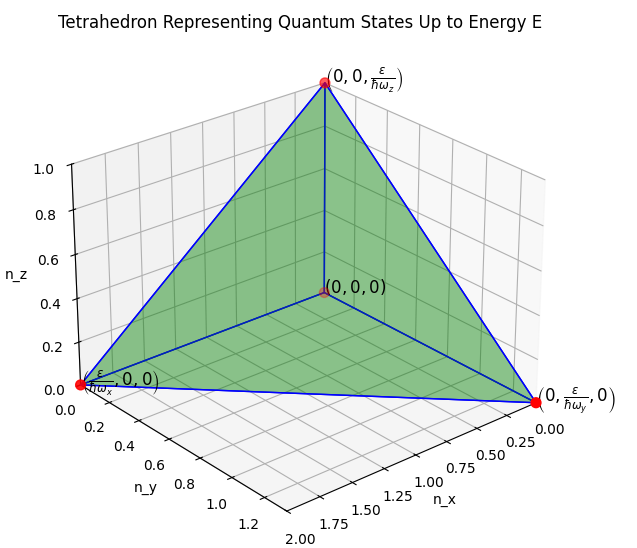
\includegraphics[width=\textwidth]{Figure_1.png}
    \end{minipage}\hfill
    \begin{minipage}{0.45\textwidth}
        \centering
        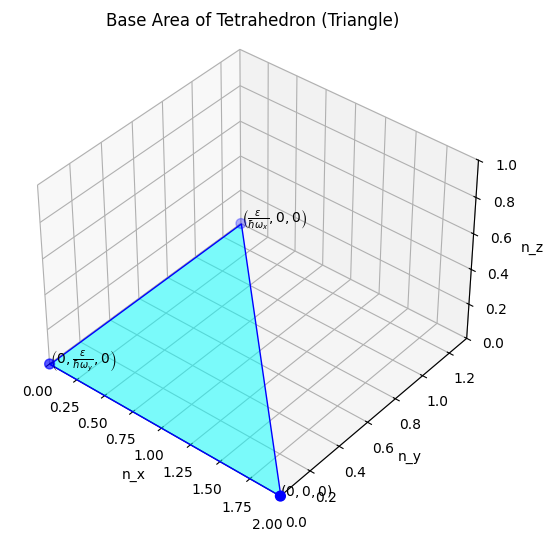
\includegraphics[width=\textwidth]{Figure_2.png}
    \end{minipage}
\end{figure}
\\
Therefore, the volume of the tetrahedron, which is the total number of states up to energy \(\varepsilon\), is
\begin{equation}
    G(\varepsilon) = \frac{\varepsilon^3}{6\hbar^3\omega_{\mathit{x}}\omega_{\mathit{y}}\omega_{\mathit{z}}}
\end{equation} 
Now let us define the geometric mean of the frequencies 
\begin{equation}
    \Omega = \sqrt[3]{\omega_{\mathit{x}}\omega_{\mathit{y}}\omega_{\mathit{z}}}
\end{equation}
And the DOS is the derivative of the total number of states with respect to \(\varepsilon\), which is
\begin{equation}
    g(\mathit{\varepsilon}) = \frac{\varepsilon^2}{2(\hbar\Omega)^3}
\end{equation} 
Note that eqn(2.3.3) is the near as eqn(2.2.7) if we consider the isotropic case, where \(\omega_{\mathit{x}} = \omega_{\mathit{y}} = \omega_{\mathit{z}} = \omega\). Under this condition, the geometric mean of the frequencies becomes:
\[
\Omega = \sqrt[3]{\omega_{\mathit{x}}\omega_{\mathit{y}}\omega_{\mathit{z}}} = \sqrt[3]{\omega^3} = \omega.
\]
Substituting this into eqn(2.3.3) for the anisotropic potential:
\[
g(\varepsilon) = \frac{\varepsilon^2}{2(\hbar \Omega)^3} \quad \longrightarrow \quad g(\varepsilon) = \frac{\varepsilon^2}{2(\hbar \omega)^3},
\]
which matches eqn(2.2.7) for the isotropic case. This shows that the two cases are equivalent when the trapping frequencies along all axes are equal.
\section{Calculating the Condensation Temperature}
To determine the condensation temperature \( T_c \) for a Bose-Einstein condensate confined in an anisotropic harmonic potential, we begin by analyzing the distribution of particles among the quantum states. At temperatures above \( T_c \), all particles occupy excited states, while below \( T_c \), a macroscopic number of particles condense into the ground state. The number of excited particles can be calculated by integrating the Bose-Einstein distribution over the density of states specific to the anisotropic trap. The condensation temperature is then obtained by equating the total number of particles \( N \) to the number of excited particles, as the ground-state population becomes negligible near \( T_c \). This calculation provides the critical temperature marking the onset of Bose-Einstein condensation.\\
The excited-state population is given by the integral of the Bose-Einstein distribution function with the density of states (DOS):
\begin{equation}
    N_{ex} = \int_{E_G}^{\infty} \frac{g(\varepsilon)}{e^{\beta (\varepsilon - \mu)} - 1} \,d\varepsilon = \frac{1}{2(\hbar\Omega)^3} \int_{E_G}^{\infty} \frac{\varepsilon^2}{e^{\beta (\varepsilon - \mu)} - 1} \,d\varepsilon,
\end{equation}
where \( \mu \) is the chemical potential.

\subsection{Introducing the Fugacity}

We now introduce the fugacity. The fugacity \( \lambda = e^{\beta \mu} \), where \( \beta = \frac{1}{k_B T} \) and \( \mu \) is the chemical potential, is a dimensionless parameter that provides insight into the thermodynamic properties of a system of particles. It quantifies the deviation of the system from ideal behavior and is particularly significant in Bose-Einstein condensation. For a system of non-interacting bosons, the fugacity is directly related to the particle distribution across quantum states.\\
When the fugacity \( \lambda < 1 \), the chemical potential \( \mu \) is negative, and the system is dominated by thermal excitations, with particles spread across many states. As \( \lambda \to 1^- \), corresponding to \( \mu \to 0^- \), the system approaches the critical conditions for Bose-Einstein condensation, where a macroscopic number of particles begin to occupy the ground state. The fugacity, therefore, serves as a critical parameter in characterizing the transition and the population of quantum states within the system.\\

\subsection{Simplifying and Solving the Integral}
To simplify the integral, we make the substitution \( x = \beta \varepsilon \), where \( \beta = \frac{1}{k_B T} \). This leads to the following transformations:
\[
\varepsilon = \frac{x}{\beta}, \quad d\varepsilon = \frac{dx}{\beta}.
\]
Substituting these into the integral:
\[
N_{ex} = \int_{E_G}^{\infty} \frac{g(\varepsilon)}{e^{\beta (\varepsilon - \mu)} - 1} \, d\varepsilon = \frac{\lambda}{2(\hbar \Omega)^3} \int_{E_G}^{\infty} \frac{\varepsilon^2}{e^{\beta \varepsilon} - 1} \, d\varepsilon.
\]
Applying the substitution:
\[
\varepsilon^2 = \left(\frac{x}{\beta}\right)^2, \quad d\varepsilon = \frac{dx}{\beta}.
\]
The integral becomes:

\[
N_{ex} = \frac{\lambda}{2(\beta \hbar \Omega)^3} \int_{x_G}^{\infty} \frac{x^2}{e^x - 1} \, dx.
\]
Assuming \( \varepsilon_G = 0 \), we set \( x_G = 0 \). The integral is now:
\[
N_{ex} = \frac{\lambda}{2(\beta \hbar \Omega)^3} \int_{0}^{\infty} \frac{x^2}{e^x - 1} \, dx.
\]
Assuming \( \varepsilon_G = 0 \), we set \( x_G = 0 \). The integral can then be computed using the following Mathematica command:
\begin{lstlisting}[language=Mathematica]
    Integrate[x^2/(Exp[x] - 1), {x, 0, Infinity}]
\end{lstlisting}
The result is:
\[
\int_{0}^{\infty} \frac{x^2}{e^x - 1} \,dx = 2\zeta(3),
\]
where \( \zeta(3) \) is the Riemann zeta function evaluated at 3. Substituting this result, we have:
\begin{equation}
    N_{ex} = \frac{\lambda}{2(\beta \hbar \Omega)^3} \cdot 2\zeta(3) = \frac{\lambda \zeta(3)}{(\beta \hbar \Omega)^3}.
\end{equation}

\subsection{Determining the Condensation Temperature}
Near the condensation temperature \( T_c \), the chemical potential \( \mu = 0 \), and thus \( \lambda = 1 \). The total number of particles is given by:
\begin{equation}
    N = N_{ex} + N_0,
\end{equation}
where \( N_0 \) is the number of particles in the ground state. Substituting for \( N_{ex} \), we find:
\begin{equation}
    N = \zeta(3) \left(\frac{k_B T}{\hbar \Omega}\right)^3 + N_0.
\end{equation}
At the critical temperature \( T_c \), the ground-state population \( N_0 \) becomes negligible, and the total number of particles is entirely in the excited states:
\begin{equation}
    N = \zeta(3) \left(\frac{k_B T_c}{\hbar \Omega}\right)^3.
\end{equation}
Solving for \( T_c \), we obtain:
\begin{equation}
    T_c = \frac{\hbar \Omega}{k_B} \left(\frac{N}{\zeta(3)}\right)^{1/3}.
\end{equation}
This is the expression for the condensation temperature, marking the onset of Bose-Einstein condensation.


\subsection{Calculating the Condensation Fraction}
The condensation fraction \( \frac{N_0}{N} \) quantifies the proportion of particles that occupy the ground state relative to the total number of particles in the system. This fraction serves as a key indicator of the onset and progression of Bose-Einstein condensation, providing insight into the redistribution of particles between the ground state and excited states as the system transitions through the critical temperature \( T_c \).
In the regime where the temperature \( T \) is below \( T_c \), a macroscopic number of particles occupy the ground state, causing the condensation fraction to increase rapidly. Near absolute zero, nearly all particles reside in the ground state, leading to \( \frac{N_0}{N} \approx 1 \). Conversely, as the temperature approaches \( T_c \), the condensation fraction diminishes, reflecting the dominance of thermal excitations over quantum effects.\\
The expression for the condensation fraction is derived by considering the total number of particles \( N \) and the number of particles in the excited states \( N_{ex} \). From Eq.~(3.0.3), the number of particles in the ground state is:
\[
N_0 = N - N_{ex},
\]
where \( N_{ex} \) represents the particles occupying excited states. Using the relationship between the total number of particles and the excited-state population, the condensation fraction is expressed as:
\[
\frac{N_0}{N} = 1 - \frac{N_{ex}}{N}.
\]
Substituting the expression for \( N_{ex} \) near the critical temperature, where \( N_{ex} = \zeta(3) \left( \frac{k_B T}{\hbar \Omega} \right)^3 \), and recalling that the condensation temperature \( T_c \) satisfies:
\[
N = \zeta(3) \left( \frac{k_B T_c}{\hbar \Omega} \right)^3,
\]
we find the condensation fraction as a function of \( T/T_c \):
\begin{equation}
    \frac{N_0}{N} = 1 - \left(\frac{T}{T_c}\right)^3.
\end{equation}
This result shows that the condensation fraction follows a cubic dependence on the temperature ratio \( T/T_c \). As \( T \) decreases below \( T_c \), the ground state population grows, reaching \( \frac{N_0}{N} \to 1 \) as \( T \to 0 \). At \( T = T_c \), \( \frac{N_0}{N} = 0 \). Thus, the relationship \( \frac{N_0}{N} = 1 - \left(\frac{T}{T_c}\right)^3 \) describes the temperature-driven transition to Bose-Einstein condensation.


\begin{center}
    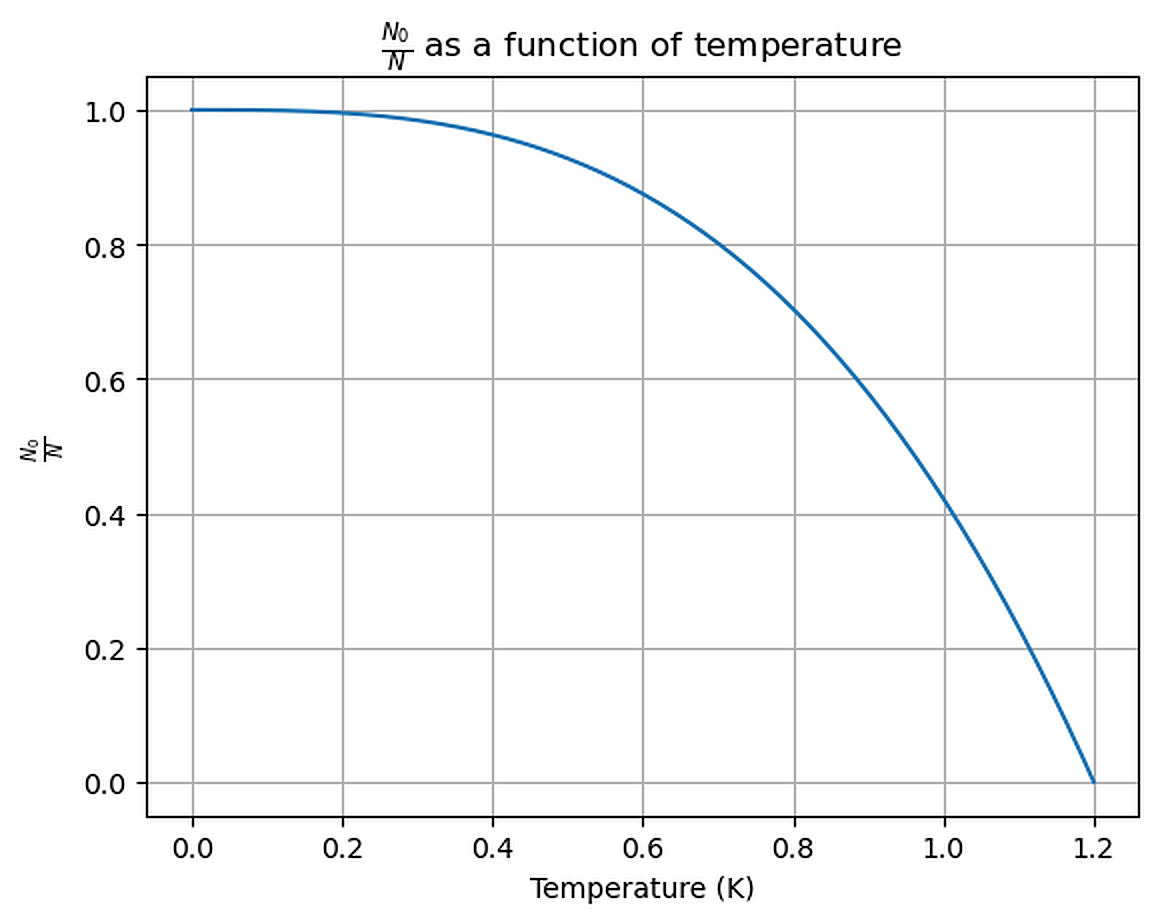
\includegraphics[width=0.7\textwidth]{N_0N_graph_high_quality.png}  
\end{center}
The graph above shows the behavior of the condensation fraction as a function of the reduced temperature \( T/T_c \) assuming $N = 10^{23}$ and $T_c = 1.2k$. Near the condensation temperature, the condensation fraction rapidly increases, approaching unity as \( T \to 0 \). 

\subsection{Chemical Potential Form}

The chemical potential \(\mu\) is a function of both temperature \(T\) and the number of particles \(N\). To maintain the particle number, we consider the relation between the number of particles in the ground state \(N_0\) and the total number of particles \(N\):
\[
\frac{N_0}{N} = 1 - \left(\frac{T}{T_c}\right)^3,
\]
where \(T_c\) is the critical temperature. Thus, the number of particles in the ground state is:
\[
N_0 = N \left( 1 - \left(\frac{T}{T_c}\right)^3 \right),
\]
and the number of particles in the excited states is:
\[
N_{\text{exc}} = N - N_0 = N \left( \frac{T}{T_c} \right)^3.
\]
Given that the chemical potential \(\mu\) adjusts to maintain the particle number in the system, it is related to the temperature \(T\) and the total number of particles \(N\). For temperatures below the critical temperature, the chemical potential \(\mu\) can be expressed as:
\[
\mu(T,N) = \hbar \Omega \left( \frac{N}{\zeta(3)} \right)^{1/3} \left( 1 - \left(\frac{T}{T_c}\right)^3 \right).
\]
This formula shows that the chemical potential decreases as the temperature approaches the critical temperature \(T_c\), where it vanishes, marking the transition to a non-condensed state.\\

\subsubsection{Chemical Potential simplified Form}

It is helpful to note that the chemical potential could also be a function of temperature at constant N and specifically, near \(T_c\), simplified it to have the form:
\[
\mu(T) = A (1 - (\frac{T}{T_c})^3),
\]
where \(A\) and \(\alpha\) are constants. This form is consistent with the fact that \(\mu\) must vanish at \(T = T_c\) and must decrease as \(T\) increases.

\subsubsection{Relation Between \(A\) and \(N\)}

The constant \(A\) reflects the scaling of the chemical potential with temperature near \(T_c\). Using the scaling relations, we can express \(A\) in terms of \(T_c\), which itself depends on \(N\). From the expression for the critical temperature \(T_c\):
\[
T_c = \frac{\hbar \Omega}{k_B} \left( \frac{N}{\zeta(3)} \right)^{1/3},
\]
and \(A\) is explicitly:
\[
    A = \hbar \Omega \left( \frac{N}{\zeta(3)}\right)^{1/3} \\
\]

we find that the constant \(A\) scales as:
\[
A \propto \frac{k_B}{T_c} \propto \frac{\Omega}{N^{1/3}}.
\]
Thus, \(A\) is inversely proportional to \(N^{1/3}\) and directly proportional to the effective trap frequency \(\Omega\). This shows that \(A\) becomes smaller for larger systems (larger \(N\)) and is influenced by the trap geometry and anisotropy through \(\Omega\).



\section{The Specific Heat}
The specific heat \( C_V \) characterizes the heat capacity of a system and provides insights into the energy required to raise the temperature by a small amount. In the context of Bose-Einstein condensation, the specific heat near the condensation temperature exhibits unique behavior, reflecting the transition from a thermal distribution to a condensed state. The specific heat is calculated by differentiating the total energy with respect to temperature, yielding the energy required to increase the temperature by a small amount.\\
$$C_V = \frac{dU}{dT}$$

\subsection{Calculating the Internal Energy}
where \( U \) is the internal energy of the system. The internal energy is given by the sum of the energy of the excited particles and the ground-state energy:
\begin{equation}
    U = \int_{\varepsilon_G}^{\infty} \varepsilon g(\varepsilon) \frac{1}{e^{\beta(\varepsilon - \mu)} - 1} \,d\varepsilon + N_0 E_0
\end{equation}
And since we assume $\varepsilon_G = 0$, the internal energy is:
\begin{equation}
    U = \int_{0}^{\infty} \varepsilon g(\varepsilon) \frac{1}{e^{\beta(\varepsilon - \mu)} - 1} \,d\varepsilon = \frac{1}{2\lambda(\hbar\Omega)^3} \int_{0}^{\infty} \frac{\varepsilon^3}{e^{\beta\varepsilon} - 1} \,d\varepsilon
\end{equation}
Now we make the substitution \( x = \beta\varepsilon\) to simplify the integral:
$$U = \frac{1}{2\lambda(\beta\hbar\Omega)^3} \int_{0}^{\infty} \frac{x^3}{e^x - 1} \,dx = \frac{1}{2\lambda\beta^4(\hbar\Omega)^3} 3!\zeta(4) = \frac{3!\zeta(4)}{2\lambda\beta^4(\hbar\Omega)^3} =   \left(\frac{3\zeta(4)}{\hbar^3\Omega^3}\right) \left(\frac{k_b^4T^4}{\lambda}\right) 
$$
Therefore, the internal energy is:
\begin{equation}
    U = \frac{3\zeta(4)}{\hbar^3\Omega^3} \left(\frac{k_b^4T^4}{\lambda}\right)
\end{equation}
where \( \zeta(4) \) is the Riemann zeta function evaluated at 4, and $\lambda = e^{\mu/k_bT}$ is the fugacity. Also near the condensation temperature, $\mu = 0$ and $\lambda = 1$, the internal energy is:   
\begin{equation}
    U_{T_c} = \frac{3\zeta(4)}{\hbar^3\Omega^3} \left(k_b^4T^4\right) 
\end{equation}
and If T is far from the condensation temperature, the internal energy is:
\begin{equation}
    U = \frac{3\zeta(4)}{\hbar^3\Omega^3} k_b^4T^4\exp\left(\frac{-\mu}{k_bT}\right)
\end{equation}


\subsection{Calculating the Specific Heat}
The specific heat near the condensation temperature is obtained by differentiating eqn(5.1.4) with respect to temperature:
\begin{equation}
    C_V = \frac{dU_{T_c}}{dT} = \frac{12\zeta(4)}{\hbar^3\Omega^3}k_b^4T^3
\end{equation}
Expressing this in terms of the reduced temperature \( T/T_c \) we get:
\begin{equation}
    C_V = \frac{12\zeta(4) N k_b}{\zeta(3)} \left(\frac{T}{T_c}\right)^3
\end{equation}
Introducing the dimensionless parameter \( x = \frac{T}{T_c} \), the specific heat is expressed as:
\begin{equation}
    C_V = \frac{12\zeta(4) N k_b}{\zeta(3)} \left(x\right)^3
\end{equation}
and far from the condensation temperature, the specific heat is obtained by differentiating eqn(5.1.5) with respect to temperature:
\begin{equation}
    C_V = \left(\frac{3\zeta(4)}{\hbar^3\Omega^3}\right) \frac{d}{dT}\left(k_b^4T^4\exp\left(\frac{-\mu}{k_bT}\right)\right) 
\end{equation}
Therefore, the specific heat is:
\begin{equation}
    C_V = \left(\frac{3\zeta(4)}{\hbar^3\Omega^3}\right) \left(4k_b^4T^3\exp\left(\frac{-\mu}{k_bT}\right) - k_b^4T^4\exp\left(\frac{-\mu}{k_bT}\right)\left(\frac{-\mu}{k_bT^2}\right)\right)
\end{equation}
After simplifying the above equation, we get:
\begin{equation}
    C_V = \left(\frac{3\zeta(4)}{\hbar^3 \Omega^3}\right) k_b^4  \left( 4T^3 + \frac{\mu}{k_b} T^2 \right) \exp\left(-\frac{\mu}{k_B T}\right)
\end{equation}
expressing this in terms of the reduced temperature \( T/T_c \) we get:
\begin{equation}
    C_V = \frac{3\zeta(4) N k_b}{\zeta(3)}  \left( 4\left(\frac{T}{T_c}\right)^3 + \frac{\mu}{k_b T_c} \left(\frac{T}{T_c}\right)^2 \right)\exp\left(-\frac{\mu}{k_b T}\right)
\end{equation}
Introducing the dimensionless parameter \( x = \frac{T}{T_c} \) and the reduced chemical potential \( \mu^* = \frac{\mu}{k_b T_c} \), the specific heat is expressed as:
\begin{equation}
    C_V = \frac{3\zeta(4) N k_b}{\zeta(3)}  \left( 4x^3 + \mu^* x^2 \right)\exp\left(-\frac{\mu^*}{x}\right)
\end{equation}
Therefore we have the specific heat:
\begin{equation}
    \frac{C_V}{N k_b} = 
\begin{cases} 
\frac{12 \zeta(4) }{\zeta(3)} \, x^3 & \text{if } x \leq 1, \\[8pt]
\frac{3 \zeta(4) }{\zeta(3)} \left( 4x^3 + \mu^* x^2 \right) \exp\left(-\frac{\mu^*}{x}\right) & \text{if } x > 1.
\end{cases}
\end{equation}

\subsection{Specific Heat Plot}
The specific heat is plotted below for  $T_c = 1k$, $\alpha = 1$, and $A = 20\ kg\ m^2\ s^{-1}$. This choice of A is related to choosing N to be $10^{4}$ and $\Omega = 1\ s^{-1}$. 
\begin{center}
    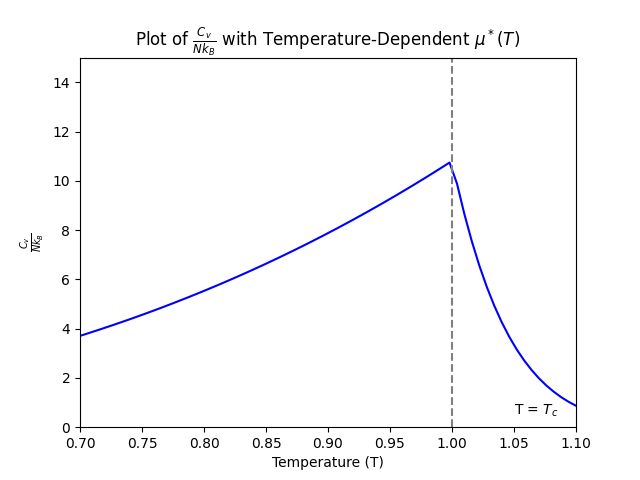
\includegraphics[width=0.7\textwidth]{Figure_3.png}
\end{center}
The specific heat exhibits a peak near the condensation temperature, reflecting the transition from a thermal distribution to a condensed state. The peak height and width depend on the number of particles and the functional form of the chemical potential.
\newpage
\section{Conclusion}

In this project, we have thoroughly investigated the behavior of a Bose-Einstein condensate (BEC) confined in anisotropic harmonic potentials. By deriving the density of states for both isotropic and anisotropic traps, we captured the critical role of trap geometry in determining the system's thermodynamic properties. The calculated condensation temperature and condensation fraction offer valuable insights into the transition to a condensed state, revealing how the ground-state population grows as the system cools below the critical temperature. Furthermore, we derived the specific heat as a function of temperature and particle number, highlighting the distinct peak near the condensation temperature, which signifies the transition from a classical thermal distribution to a macroscopic quantum state.

These findings not only provide a detailed theoretical framework for understanding BEC in anisotropic traps but also emphasize the significance of key factors such as particle number, trap geometry, and anisotropy in shaping condensation dynamics. The results presented herein contribute to a deeper understanding of BEC phenomena and form a robust foundation for future theoretical and experimental investigations into quantum systems.

\section{Further Discussion}

This study opens avenues for several promising research directions. One important extension involves considering finite-size effects, which could uncover deviations from the thermodynamic limit, particularly near the critical temperature \(T_c\). Another crucial aspect is the inclusion of interatomic interactions among bosons, which would offer a more realistic representation of experimental systems and refine the understanding of collective quantum behavior. Additionally, exploring BEC in lower-dimensional traps, such as one-dimensional or two-dimensional configurations, could illuminate the role of dimensionality in quantum coherence and condensation dynamics.

Comparative analysis with experimental data, especially for highly anisotropic traps, would be instrumental in validating theoretical assumptions about density of states and specific heat. Such experimental correlations could help refine the theoretical models and adapt them to real-world applications. Lastly, investigating non-equilibrium dynamics, such as the time-dependent formation and coherence of the condensate, could provide insights into transient phenomena and quantum phase transitions. These directions collectively highlight the potential for expanding our understanding of Bose-Einstein condensation and its implications for both fundamental quantum physics and practical applications in quantum technologies.


\section{References}
\begin{enumerate}
    \item H. Haugerud, T. Haugset, and F. Ravndal, “A more accurate analysis of Bose-Einstein condensation in harmonic traps,” \textit{Physics Letters A}, vol. 225, no. 1–3, pp. 18–22, Jan. 1997. doi: \url{https://doi.org/10.1016/s0375-9601(96)08842-1}.
    \item T. Haugset, H. Haugerud, and J. O. Andersen, “Bose-Einstein condensation in anisotropic harmonic traps,” \textit{Physical Review A}, vol. 55, no. 4, pp. 2922–2929, Apr. 1997. doi: \url{https://doi.org/10.1103/physreva.55.2922}.
    \item F. Dalfovo, S. Giorgini, L. P. Pitaevskii, and S. Stringari, “Theory of Bose-Einstein condensation in trapped gases,” \textit{Reviews of Modern Physics}, vol. 71, no. 3, pp. 463–512, Apr. 1999. doi: \url{https://doi.org/10.1103/revmodphys.71.463}.
    \item S. Grossmann and M. Holthaus, “On Bose-Einstein condensation in harmonic traps,” \textit{Physics Letters A}, vol. 208, no. 3, pp. 188–192, Nov. 1995. doi: \url{https://doi.org/10.1016/0375-9601(95)00766-v}.
    \item K. Kirsten and D. J. Toms, “Bose-Einstein condensation of atomic gases in a general harmonic-oscillator confining potential trap,” \textit{Physical Review A}, vol. 54, no. 5, pp. 4188–4203, Nov. 1996. doi: \url{https://doi.org/10.1103/physreva.54.4188}.
    \item M. Edwards, R. J. Dodd, C. W. Clark, P. A. Ruprecht, and K. Burnett, “Properties of a Bose-Einstein condensate in an anisotropic harmonic potential,” \textit{Physical Review A}, vol. 53, no. 4, pp. R1950–R1953, Apr. 1996. doi: \url{https://doi.org/10.1103/physreva.53.r1950}.
\end{enumerate}

\end{document}
